\chapter{Integración con la base de datos real}

\section{Modelo de datos}

La base de datos \texttt{InventarioProductosDB} contiene la tabla \texttt{dbo.Productos}:

\begin{table}[H]
  \centering
  \caption{Esquema relacional \texttt{dbo.Productos}}
  \begin{tabular}{@{}lll@{}}
    \toprule
    \textbf{Columna} & \textbf{Tipo} & \textbf{Restricción} \\
    \midrule
    \texttt{id} & \texttt{INT} & \texttt{PRIMARY KEY} \\
    \texttt{nombre} & \texttt{NVARCHAR(120)} & \texttt{NOT NULL} \\
    \texttt{categoria} & \texttt{NVARCHAR(80)} & \texttt{NOT NULL} \\
    \texttt{precio} & \texttt{DECIMAL(10,2)} & \texttt{NOT NULL} \\
    \texttt{stock} & \texttt{INT} & \texttt{NOT NULL} \\
    \bottomrule
  \end{tabular}
\end{table}

\begin{lstlisting}[style=gocode,caption={Struct Go \texttt{Product}},label={lst:product}]
type Product struct {
    ID       int
    Name     string
    Category string
    Price    float64
    Stock    int
}
\end{lstlisting}

\section{Conexión Go $\leftrightarrow$ SQL Server}

Driver: \texttt{github.com/denisenkom/go-mssqldb}. Configuración vía variables de entorno (\texttt{SQLSERVER\_HOST}, \texttt{SQLSERVER\_DATABASE}, etc.) o \texttt{SQLSERVER\_DSN}. Pool: \texttt{MaxOpenConns(5)}, \texttt{ConnMaxIdleConns(5)}, timeout de 10~s en \texttt{PingContext}.

\section{Estrategia de carga}

\begin{enumerate}
  \item \texttt{ListProducts(ctx, db)} $\rightarrow$ \texttt{SELECT ... ORDER BY id}.
  \item Para cada \texttt{Product}: \texttt{tree.Insert(product.ID, product)}.
\end{enumerate}

\begin{lstlisting}[style=gocode,caption={Carga de productos al índice en memoria}]
for _, product := range products {
    index.Insert(product.ID, product)
}
\end{lstlisting}

\section{Rol del \Scapegoat{} sobre datos persistidos}

SQL Server resuelve persistencia; el \Scapegoat{} en RAM actúa como \textbf{índice ordenado por \texttt{id}} con búsqueda $\bigO(\log n)$ amortizada y recorrido \texttt{InOrder()} en $\bigO(n)$.

\begin{figure}[H]
  \centering
  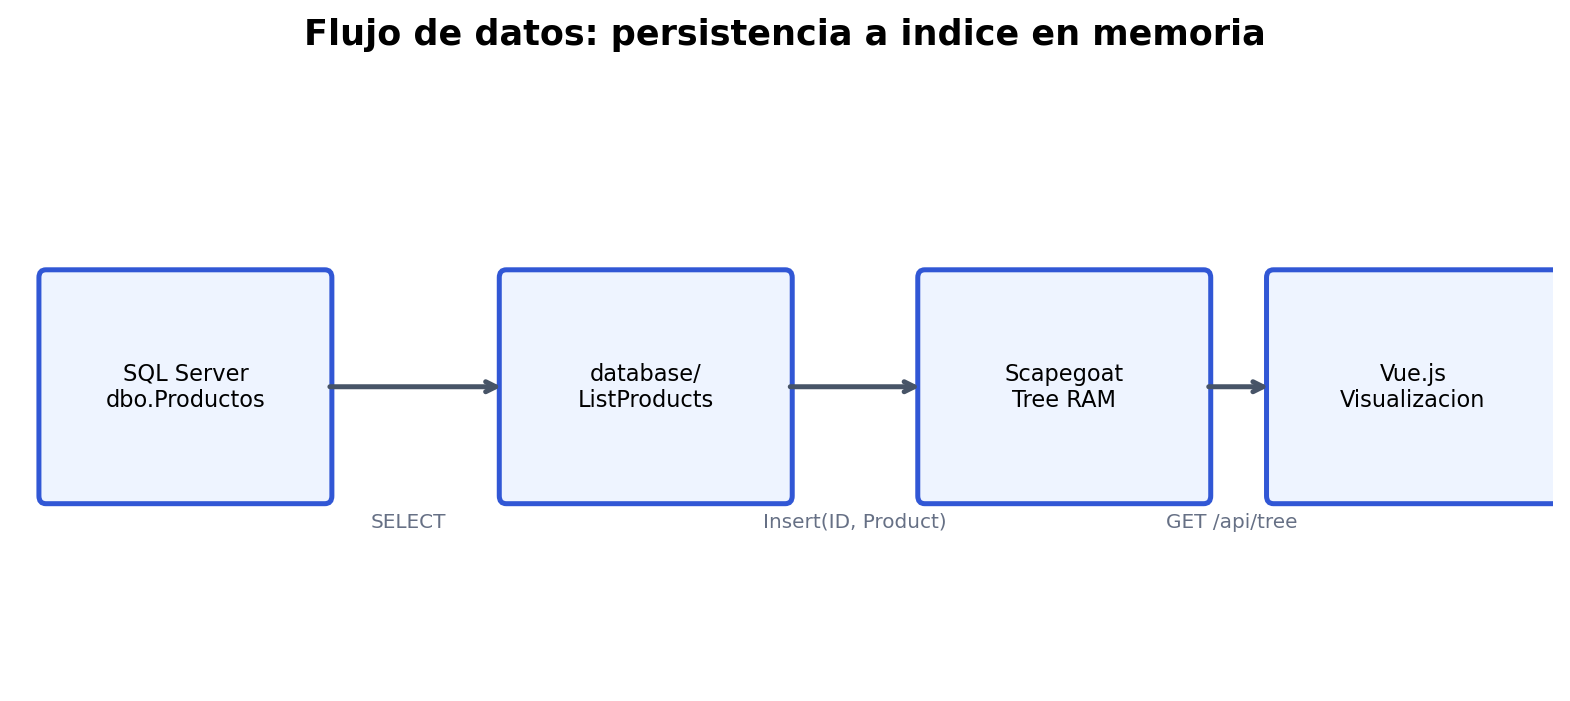
\includegraphics[width=0.92\textwidth]{diagrams/03-flujo-datos.png}
  \caption{Flujo de datos desde SQL Server al índice en memoria}
  \label{fig:flujo-datos}
\end{figure}

\begin{figure}[H]
  \centering
  \begin{tikzpicture}[
    actor/.style={rectangle, draw, rounded corners, minimum width=2cm, minimum height=0.7cm, align=center, font=\footnotesize},
    arrow/.style={-{Stealth[length=2mm]}, thick}
  ]
    \node[actor] (ss) {SQL Server};
    \node[actor, right=1.2cm of ss] (db) {database/};
    \node[actor, right=1.2cm of db] (api) {API Go};
    \node[actor, right=1.2cm of api] (st) {Scapegoat};
    \node[actor, right=1.2cm of st] (ui) {Vue.js};
    \draw[arrow] (ss) -- node[above] {SELECT} (db);
    \draw[arrow] (db) -- node[above] {[]Product} (api);
    \draw[arrow] (api) -- node[above] {Insert} (st);
    \draw[arrow] (st) -- node[above] {JSON} (ui);
  \end{tikzpicture}
  \caption{Secuencia de integración con base de datos}
  \label{fig:seq-db}
\end{figure}
